\section{Countermeasures placement}

\subsection{Introduction}

\begin{frame}[fragile]{Placement of software countermeasures}
    \begin{columns}
        \begin{column}{0.55\textwidth}    
            \lstset{style=customc, escapeinside={(*}{*)}}
            \begin{lstlisting}
bool compare(uchar* a1, uchar* a2, size_t size)
{
    bool ret = true;
    size_t i = 0; 
    for(; i < size; i++) {
        
        if(a1[i] != a2[i]) {
            ret = false;
        }
    }
        
    return ret;
}
            \end{lstlisting}	
            \vfill
        \end{column}
        \begin{column}{0.55\textwidth}
            \begin{small}
                \begin{itemize}
                    \item \textbf{Goal}: help to place countermeasures in multiple fault context (P2 and P3)
                    \item[] $\rightarrow$ several fault models can be considered
                    \item[] $\rightarrow$ countermeasures can be attacked with each fault model
                    \item[] $\rightarrow$ countermeasures can introduce attacks
                    \item[] $\rightarrow$ using a defined attack objective
                \end{itemize}
            \end{small}
        \vfill
        \end{column}
    \end{columns}
\end{frame}

\begin{frame}[fragile, noframenumbering]{Placement of software countermeasures}
    \begin{columns}
        \begin{column}{0.55\textwidth}
            \lstset{style=customc, escapeinside={(*}{*)}}
            \begin{lstlisting}
bool compare(uchar* a1, uchar* a2, size_t size)
{
    bool ret = true;
    size_t i = 0; 
    for(; i < size; i++) {
        (*{\color{mauve} if(i >= size) killcard();}*) // Duplication (true)
        (*{\color{mauve} if(i >= size) killcard();}*) // Triplication (true)

        (*{\color{mauve} uchar a1\_dup = a1[i]; }*) // Load duplication
        (*{\color{mauve} if(a1\_dup != a1[i]) killcard(); }*)
        (*{\color{mauve} uchar a2\_dup = a2[i]; }*) // Load duplication
        (*{\color{mauve} if(a1\_dup != a1[i]) killcard(); }*) 
        
        if(a1[i] != a2[i]) {
            (*{\color{mauve} if(i >= size) killcard();}*) // Duplication (true)
            (*{\color{mauve} if(i >= size) killcard();}*) // Triplication (true)
            ret = false;
        }
    }
    (*{\color{mauve} if(i != size) killcard();}*) // Duplication (false)
    (*{\color{mauve} if(i != size) killcard();}*) // Triplication (false)
        
    return ret;
}
            \end{lstlisting}	
            \vfill
        \end{column}
        \begin{column}{0.55\textwidth}
    	   \begin{small}
                 \begin{itemize}
                     \item \textbf{Goal}: help to place countermeasures in multiple fault context (P2 and P3)
                     \item[] $\rightarrow$ several fault models can be considered
                     \item[] $\rightarrow$ countermeasures can be attacked with each fault model
                     \item[] $\rightarrow$ countermeasures can introduce attacks
                     \item[] $\rightarrow$ using a defined attack objective
                 \end{itemize}
    	   \end{small}
            \vfill
        \end{column}
    \end{columns}
\end{frame}

\begin{frame}[fragile]{Placement of software countermeasures} 
    \textbf{Goal}: help to place countermeasures in multiple fault context 
    
    \begin{itemize}
        \item Target robustness in $N$ faults
        \item Give guarantees even if trace exploration is not complete
        \item Using a catalog of countermeasures schemes with \textit{Injection Point} (IP) granularity 
        \item []
    \end{itemize}

    \textbf{Approach:}
    \begin{itemize}
        \item  Compositional analysis using:
        \begin{itemize}
            \item  \textit{Isolation analysis} of countermeasures schemes
            \item[] $\rightarrow$ Notion of protection coefficient
            \item Exploration of attacks traces on the program P
        \end{itemize}        
        \item Placement algorithms
    \end{itemize}
\vfill
\end{frame}

\subsection{Analysis in isolation}

\begin{frame}[fragile]{Principle of analysis in isolation}
    \begin{columns}
        \begin{column}{0.2\textwidth}
            \begin{figure}
                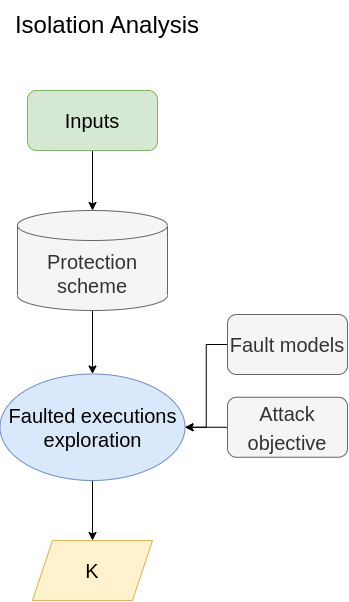
\includegraphics[scale=0.25]{img/out-of-context-metho.png}
            \end{figure}
    	\vfill
        \end{column}
        \begin{column}{0.04\textwidth} \end{column}
        \begin{small}
            \begin{column}{0.75\textwidth}
                \begin{itemize}
                    \item Analysis of countermeasures scheme in isolation
                    \item Focus on countermeasures with IP granularity
                    \item[] $\rightarrow$ A \textbf{protection scheme} describe how an IP is protected
                    \item Research of the \textit{protection coefficient} (K) of the protection scheme:
                    \item[] $\rightarrow$ e.g. \textit{How many faults are required to induce an abnormal behavior (not detected) for the protected IP ?}
                    \item[] $\rightarrow$ Unprotected IP has a $K = 1$
                    \item[] $\rightarrow$ Can be computed with Lazart 
                \end{itemize}
            \end{column}             
        \end{small}
    \end{columns}
\end{frame}

\begin{frame}[fragile]{Analysis in isolation of Branch duplication scheme}
    \begin{columns}
        \begin{column}{0.25\textwidth}
            \begin{figure}
                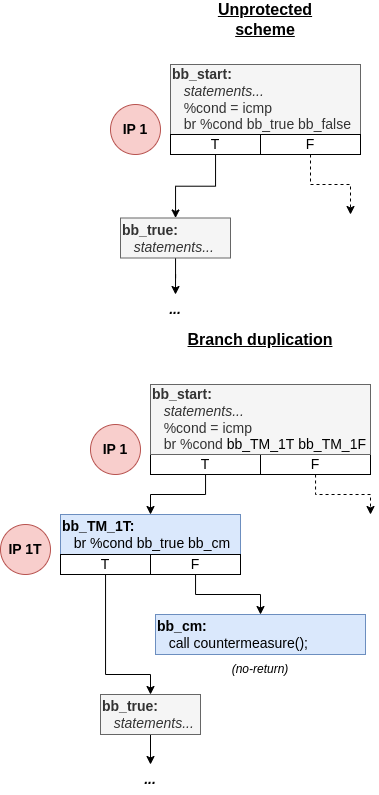
\includegraphics[scale=0.25]{img/branch-mul.png}
            \end{figure}
            \vfill
        \end{column}
        \begin{column}{0.04\textwidth} \end{column}
        \begin{small}
            \begin{column}{0.7\textwidth}
                Branch Multiplication ($BM_n$): n-plication of a conditional branch
                \vspace{0.3cm}
                
                Isolation analysis with \textit{Branch Inversion} fault model                
                \vspace{0.3cm}
                
                \onslide<2-> {
                    Need to define:
                    \begin{itemize}
                        \item Input(s) of the scheme
                        \onslide<3->{$\rightarrow$ \textbf{the \texttt{\%cond} temporary}}
                        \item Output(s) of the scheme \onslide<3->{$\rightarrow$ \textbf{the destination branch}}
                        \item Entry point(s) \onslide<4->{$\rightarrow$ \textbf{the \texttt{br} instruction (\texttt{bb\_start})}}
                        \item Output point(s) \onslide<4->{$\rightarrow$ \textbf{the destination block (\texttt{bb\_true})}}
                        \item Attack surface \onslide<5->{$\rightarrow$ \textbf{$IP\; 1$ and $IP\; 1T$ with BI fault model}}
                        \item Nominal behavior \onslide<6->{$\rightarrow$ \textbf{reach \texttt{bb\_true} if and only if \%cond is true}}
                    \end{itemize}
                }
            \end{column}
        \end{small}
    \end{columns}
\end{frame}

\begin{frame}[fragile]{Analysis in isolation of BM schemes}
    \begin{columns}
        \begin{column}{0.45\textwidth}
            \begin{figure}
                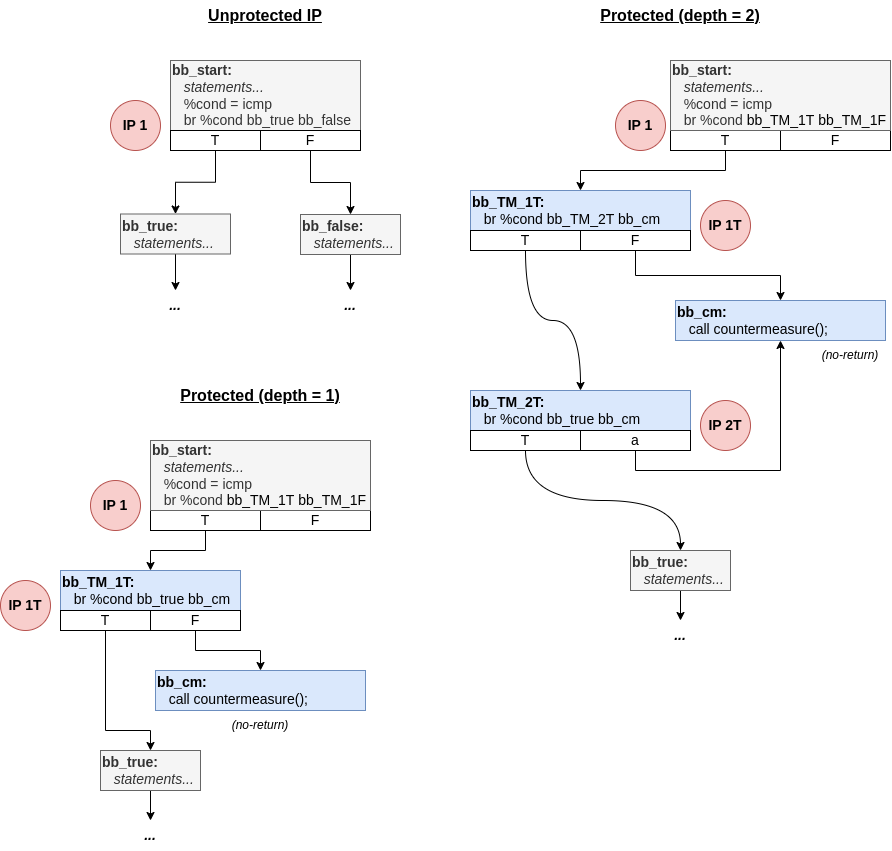
\includegraphics[scale=0.20]{img/cm-mul-test-large.png}
            \end{figure}
            \vfill
        \end{column}
        \begin{column}{0.07\textwidth} \end{column}
        \begin{small}
            \begin{column}{0.48\textwidth}
                \textbf{Branch Multiplication} ($BM_n$): n-plication of a conditional branch                
                \vspace{0.3cm}
                
                Isolation analysis with \textit{Branch Inversion} fault model
                \vspace{0.3cm}
        
                \begin{table}[ht]
                    \begin{tiny}
                        \begin{center}
                            \setlength\tabcolsep{2.1pt} % default value: 6pt
                            \begin{tabular}{l|ccccc}
                                Countermeasure & 0-faults & 1-fault & 2-faults & 3-faults  & \textbf{$K$} \\
                                \hline
                                $BM_0$ & 0 & 1 & 0 & 0 & \textbf{1}\\
                                $BM_1$ & 0 & 0 & 1 & 0 & \textbf{2} \\
                                $BM_2$ & 0 & 0 & 0 & 1 & \textbf{3}
                            \end{tabular}
                        \end{center}                         
                    \end{tiny}
                    \caption{$BM$ isolation analysis}
                \end{table}
            \end{column}
        \end{small}
    \end{columns}
\end{frame}

\begin{frame}[fragile]{Analysis in isolation of LM schemes}
    \begin{columns}
        \begin{column}{0.35\textwidth}
            \begin{figure}
                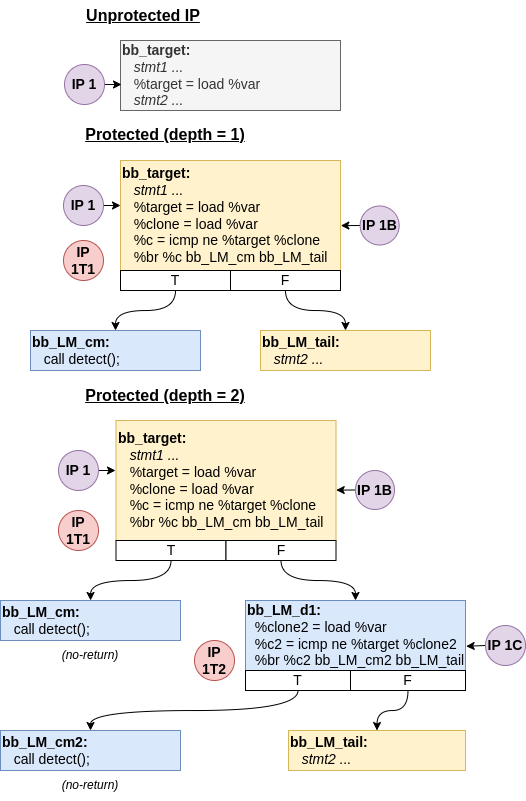
\includegraphics[scale=0.24]{img/cm-mul-load-full-sepend.drawio.png}
            \end{figure}
            \vfill
        \end{column}
        \begin{column}{0.01\textwidth} \end{column}
        \begin{small}
            \begin{column}{0.65\textwidth}            
                \textbf{Load Multiplication} ($LM_n$): n-plication of a \texttt{load} instruction (and checks)
                    
                \begin{itemize}
                    \item []
                \end{itemize}
                
                Isolation analysis with \textit{Data Load} and \textit{Branch Inversion} fault models
                \vspace{0.2cm}
                
                \begin{itemize}
                    \item Input: the value stored in \texttt{\%var} memory cell
                    \item Output: the value loaded in \texttt{\%target}
                    \item Nominal behavior: \texttt{\%target} stores \texttt{\%var}'s value
                \end{itemize}
                
                \begin{table}[ht]
                    \begin{tiny}
                        \begin{center}
                            \setlength\tabcolsep{2.1pt}
                            \begin{tabular}{l|ccccc}
                                Countermeasure & 0-faults & 1-fault & 2-faults & 3-faults &  \textbf{$K$} \\
                                \hline
                                $LM_0$ & 0 & 1 & 0 & 0 &  \textbf{1}\\
                                $LM_1$ & 0 & 0 & 1 & 0 &  \textbf{2} \\
                                $LM_2$ & 0 & 0 & 0 & 1 &  \textbf{3}
                            \end{tabular}
                        \end{center} 
                    \end{tiny}
                    \caption{$LM$ isolation analysis}
                \end{table}
            \end{column}
        \end{small}
    \end{columns}
\end{frame}

\subsection{Placement algorithms}

\begin{frame}[fragile]{Placement algorithms principles}
	\begin{small}
        \textbf{GOAL:} generate a P' program which is robust to $N$ faults
        \vspace{0.25cm}
        
        $\Rightarrow$ Give guarantees that P' is \textit{more robust than P} even if trace set is \textit{incomplete} or if catalog is incomplete
        \vspace{0.45cm}
        
        \onslide<2->{
            Basic structure of placement algorithms:
            \begin{enumerate}
                \item Obtain set of attack traces
                \item[] $\Rightarrow$ Computed with all fault models and the user-defined attack objectives
                \item Compute \textbf{required protection coefficient} ($K_{ip}$) for each IP (initialized to 1)
                \item Generate $P'$ with protection scheme matching the \textbf{required protection coefficients}
                \item[] $\Rightarrow$ Using a catalog $\mathcal{C}$ of countermeasures (with computed $K_{ip}$)
            \end{enumerate}        
        \vspace{0.5cm}
        }
        \onslide<3>{
            Three approaches:
            \begin{itemize}
                \item \textit{Systematic} placement: protect all IPs of a set with K > N
                \item \textit{Block} placement: protect at least one IPs of all attacks with K > N
                \item \textit{Distributed} placement: protect IPs such as for each trace, the sum of K of each IP is greater than N
            \end{itemize}
        }        
        \vfill
	\end{small}
\end{frame}

\begin{frame}[fragile]{Systematic placement algorithms}
    \begin{columns}
        \begin{column}{0.5\textwidth}
            \begin{tiny}
                \lstset{style=custompython}
                \begin{lstlisting}
def placement_min(C: Catalog, P: Program, M: AttackModel, n: int):
    # Get sucessfull non-detected attacks.
    attacks = T_s(P, M, n)
    # Filter with minimals attacks.
    minimals = RedundacyAnalysis(attacks).minimals()
    
    # Initial protection factors Kn at 1 for all IP.
    required_kn = { IPA: 1, IPB: 1, ..., IPN: 1 }

    # Apply ponderation of n for all IP in traces
    for attack in minimals:
        for IP in attack:
            required_kn[IP] = n + 1 # Make IP robust en n faults.

    # Generation of P'
    P` = P
    for IP, kn in required_kn:
        S = C.get_cm(IP.model(), kn) # Select protection scheme from catalog
        P` = S(P`, IP) # Apply local protection        
    return P`    \end{lstlisting}
            \end{tiny}
        \end{column}
        \begin{column}{0.5\textwidth}
            \begin{tiny}
                \textbf{Systematic algorithms:}
                \begin{itemize}
                    \item Naive placement (\texttt{naive}): protect all IP with K > N
                    \item [] $\rightarrow$ \textit{corresponds to standards systematic protection tools}% \cite{ Lalande/ESORICS14, Ferriere/LLVM19}}
                    \item [] $\rightarrow$ do not require attacks paths
                    \item Attack placement (\texttt{atk}): protect all IP in attacks with K > N
                    \item Minimal placement  (\texttt{min}) (\textbf{on left)}: protect all IP in minimal attacks with K > N
                \end{itemize}
                
                \vspace{0.6cm}
                \onslide<2-> {
                    Guarantees:
                    \begin{itemize}
                        \item \textbf{Robust in $N$ faults} if the catalog provides required $K$ for each IP (complete catalog) and if the entry trace set is complete
                        \onslide<3->{\item \textbf{At least as robust as $P$} otherwise}
                        \onslide<3->{\item[] $\rightarrow$ if the catalog is incomplete, \textit{vulnerable traces in $P'$ are known}}
                    \end{itemize}
                }
                \vfill
            \end{tiny}
        \end{column}
    \end{columns}
\end{frame}

\begin{frame}[fragile]{Block placement algorithm}
    \begin{columns}
        \begin{column}{0.5\textwidth}
            \begin{tiny}
                \lstset{style=custompython}
                \begin{lstlisting}
def placement_bloc_h(C: Catalog, P: Program, M: AttackModel, n: int):
    # Get sucessfull non-detected attacks.
    attacks = T_s(P, M, n)
    # Filter with minimals attacks.
    minimals = RedundacyAnalysis(attacks).minimals()
    
    # Initial protection factors Kn at 1 for all IP.
    required_kn = { IPA: 1, IPB: 1, ..., IPN: 1 }
            
    # For all attacks by faults count.
    for order in 1 to n:
        # Loop trought order-faults attacks by number of associated redundant attacks.
        for attack in minimals.where(order=order).sort_by(Minimals):
            if is_protected(attack, required_kn):
                continue
            # Make attack robust in n faults
            IP = select IP in attack with most occurence
            required_kn[IP] = n + 1

    # Generation of P'
    P` = P
    for IP, kn in required_kn:
        S = C.get_cm(IP.model(), kn) # Select protection scheme from catalog
        P` = S(P`, IP) # Apply local protection        
    return P`   \end{lstlisting}
            \end{tiny}
        \end{column}
        \begin{column}{0.5\textwidth}
        	\begin{tiny}
                Protection of at least one IP per minimal attack with K > N
                \begin{itemize}
                    \item [] $\rightarrow$ heuristic based
                \end{itemize}
                \vspace{0.6cm}
                
                Guarantees:
                \begin{itemize}
                    \item \textbf{Robust in $N$ faults} if the catalog provides required $K$ for each IP (complete catalog) and if the entry trace set is complete
                    \item \textbf{At least as robust as $P$} otherwise
                    \item[] $\rightarrow$ if the catalog is incomplete, \textit{vulnerable traces in $P'$ are known}
                \end{itemize}
                \vspace{1cm}
                \textit{How to be sure than no attack paths is introduced by non-protected IPs ?}
                
                \vfill
        	\end{tiny}
        \end{column}
    \end{columns}
\end{frame}

\begin{frame}[fragile]{Compositional analysis placement}
    \begin{columns}
        \begin{column}{0.6\textwidth}
            \begin{figure}
                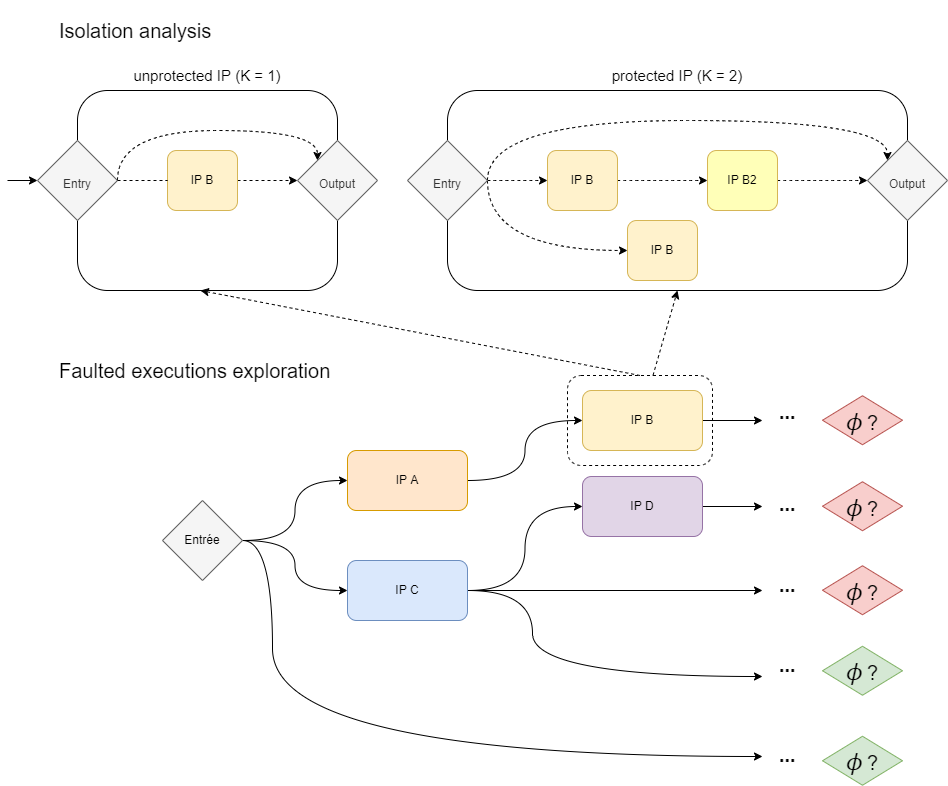
\includegraphics[scale=0.21]{img/placement-isolation-end.drawio.png}
            \end{figure}
        \end{column}
        \begin{column}{0.4\textwidth}
            \begin{tiny}
                \begin{itemize}
                    \item Isolation analysis for each considered protection scheme with all studied fault models                
                    \item []
                    \item []
                    \item []
                    \item []                
                    \item Attacks traces gives guarantees on which IP violation can lead to an attack
                    \item [] $\rightarrow$ \textit{Here, $IP A$ can be left unprotected if $IP B$ is protected}
                    \item []
                \end{itemize}
    
                \onslide<2>{
                    $\Rightarrow$ \textbf{Protection can be distributed between the IPs }
                }
            \end{tiny}
        \end{column}
\end{columns}
\end{frame}

\begin{frame}[fragile]{Optimal distributed placement} 
    \begin{tiny}
        \begin{itemize}
            \item  Distribute protections of IPs inside minimal attacks traces to ensure at least N + 1 faults are required to obtain attacks
            \item[] $\rightarrow$ usable if the catalog $\mathcal{C}$ does not contains CM for K > N
            \item[]
            \item An Integer Linear Programming (ILP) optimization problem 
            \item[] $\rightarrow$ attacks gives constraints on the protection to apply
        \end{itemize}
        
        \begin{figure}
            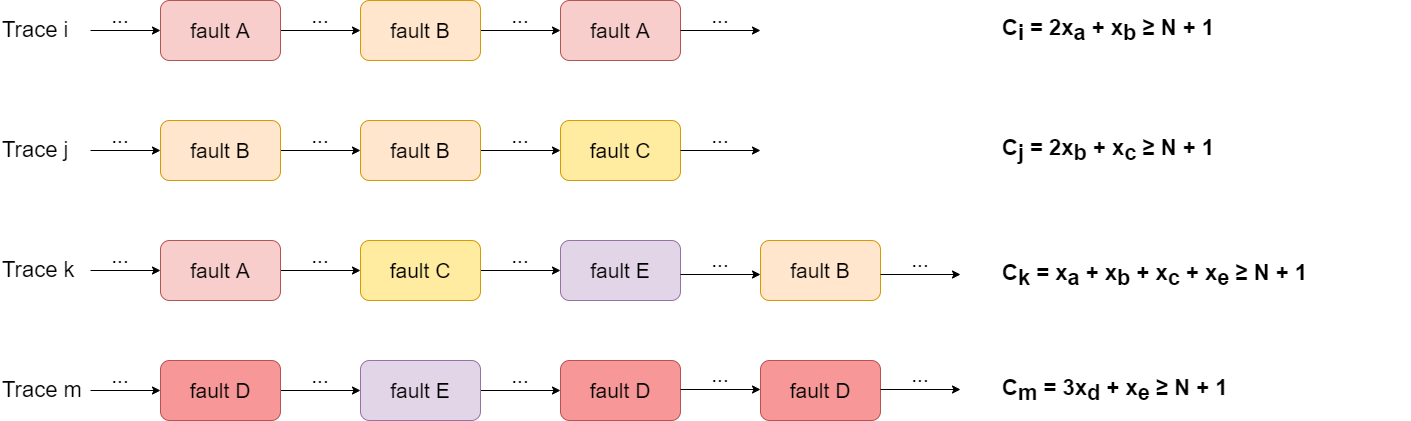
\includegraphics[scale=0.18]{img/placement-eq.drawio.png}
        \end{figure}
        
        \begin{itemize}
            \item[]
            \item[] Research of the \textbf{optimal} placement
            \item[] $\Rightarrow$ minimize the protection weight $Z = x_a + x_b + ... + x_p$
            \item[]
            \item require to ensure that all states produced by the protected IPs are studied in trace exploration fault models 
            \item[] $\rightarrow$ \textit{guarantees on partially protected IPs}
        \end{itemize}
    \end{tiny}
\end{frame}

\begin{frame}[fragile]{Optimal distributed placement}
    \begin{columns}
        \begin{column}{0.5\textwidth}
            \begin{tiny}
                \lstset{style=custompython}
                \begin{lstlisting}
def placement_rep_opt(C: Catalog, P: Program, M: AttackModel, n: int):
    # Get sucessfull non-detected attacks.
    attacks = T_s(P, M, n)
    # Filter with minimals attacks.
    minimals = RedundacyAnalysis(attacks).minimals()
    
    # Initial protection factors Kn at 1 for all IP.
    required_kn = { IPA: 1, IPB: 1, ..., IPN: 1 }
    
    constraints = [] # constraints for ILP
    for attack in minimals:
        constraints += compute_constraint(attack)
    
    required_kn = solve_ilp(constraints, required_kn)
    
    # Generation of P'
    P` = P
    for IP, kn in required_kn:
        S = C.get_cm(IP.model(), kn) # Select protection scheme from catalog
        P` = S(P`, IP) # Apply local protection        
    return P`   \end{lstlisting}
            \end{tiny}
        \end{column}
        \begin{column}{0.5\textwidth}
            \begin{tiny}
                Optimal placement using ILP problem encoding:
                \begin{enumerate}
                    \item Encode constraints from attack traces (lines 10-12)
                    \item Solve ILP (line 14)
                    \item Generate P' (lines 17-20)
                \end{enumerate}
    
                \vspace{0.6cm}
                Guarantees:
                \begin{itemize}
                    \item \textbf{Robust in $N$ faults} if the catalog provides required $K$ for each IP (complete catalog) and if the entry trace set is complete
                    \item[] $\rightarrow$ and \textbf{optimal} (i.e. minimal set of protections wrt $\mathcal{C}$) 
                    \item \textbf{At least as robust as $P$} otherwise
                    \item[] $\rightarrow$ if the catalog is incomplete, \textit{vulnerable traces in $P'$ are known}
                \end{itemize}        
                \vfill
            \end{tiny}
        \end{column}
    \end{columns}
\end{frame}

\subsection{Experimentation}

\begin{frame}{Experimentation - verify\_pin} 
    \begin{small}
        \textit{verify\_pin} \cite{Dureuil/PPLCC16} (\textbf{VP}): smart-card PIN verification process
        
        \begin{itemize}
             \item \textit{fault model:} branch inversion
             \item \textit{inputs:} input PINs are different and symbolic
             \item \textit{attack objective:} being authenticated or do not decrement the try counter 
             \item \textit{countermeasures:}
             \begin{itemize}
                 \item \textit{integrated:} hardened boolean, fixed time loop
                 \item \textit{placement:} branch multiplication (BM)
             \end{itemize}
        \end{itemize}
    \end{small}
    
    \begin{table}[htp]
        \begin{tiny}
            \begin{center}
                \begin{tabular}{lll|l|llll|l}
                \multicolumn{3}{c}{Exp.} & \multicolumn{1}{c}{Algo.} & \multicolumn{4}{c}{$\sum$ of protections} & \multicolumn{1}{c}{Robust} \\
                \hline
                Program & Fault Model & IPs &  & 1-fault & 2-faults & 3-faults & 4-faults &  \\
                \hline
                \hline
                \texttt{vp2b} & BI & \multicolumn{1}{r|}{8} & naive & 8 & 16 & 24 & 32 & \checkmark \\
                 &  &  & atk & \textbf{3} & 8 & 12 & 16 & \checkmark \\
                 &  &  & min & \textbf{3} & 8 & 12 & 16 & \checkmark \\
                 &  &  & block & \textbf{3} & \textbf{6} & \textbf{9} & \textbf{12} & \checkmark \\
                 &  &  & opt & \textbf{3} & \textbf{6} & \textbf{9} & \textbf{12} & \checkmark
                \end{tabular}
            \end{center}
        \end{tiny}
    \end{table}
\vfill
\end{frame}

\begin{frame}{Experimentations - FU1} 
    \begin{small}
        \textit{firmware\_updater} v1 (\textbf{fu1}): updates a firmware from remote source
        \begin{itemize}
            \item \textit{fault model:} branch inversion + data load
            \item \textit{inputs:} input PINs are different and symbolic
            \item \textit{attack objective:} load a corrupted firmware or avoid load
            \item \textit{countermeasures:}
            \begin{itemize}
                \item \textit{integrated:} systematic tests duplication
                \item \textit{placement:} branch multiplication (BM) and load multiplication (LM)
            \end{itemize}
        \end{itemize}
    \end{small}
    
    \begin{table}[htp]
        \begin{tiny}
            \begin{center}
            \begin{tabular}{lll|l|llll|l}
                \multicolumn{3}{c}{Exp.} & \multicolumn{1}{c}{Algo.} & \multicolumn{4}{c}{$\sum$ of protections} & \multicolumn{1}{c}{Robust} \\
                \hline
                Program & Fault Model & IPs &  & 1-fault & 2-faults & 3-faults & 4-faults &  \\
                \hline
                \hline
                \texttt{fu1} & BI & \multicolumn{1}{r|}{42} & naive & 42 & 84 & 126 & 168 & \checkmark \\
                &  &  & atk & \textbf{0} & 28 & 42 & 88 & \checkmark \\
                &  &  & min & \textbf{0} & 28 & 42 & 72 & \checkmark \\
                &  &  & block & \textbf{0} & 14 & 21 & 28 & \checkmark \\
                &  &  & opt & \textbf{0} & \textbf{7} & \textbf{14} & \textbf{21} & \checkmark \\
                \hline
                & DL & \multicolumn{1}{r|}{2} & naive & 2 & 4 & 6 & 8 & \checkmark \\
                &  &  & atk & 1 & 4 & 6 & 8 & \checkmark \\
                &  &  & min & \textbf{1} & \textbf{2} & \textbf{3} & \textbf{4} & \checkmark \\
                &  &  & block & \textbf{1} & \textbf{2} & \textbf{3} & \textbf{4} & \checkmark \\
                &  &  & opt & \textbf{1} & \textbf{2} & \textbf{3} & \textbf{4} & \checkmark \\
                \hline
                & BI+DL & \multicolumn{1}{r|}{44} & naive & 44 & 88 & 132 & 176 & \checkmark \\
                &  &  & atk & \textbf{1} & 32 & 60 & 96 & \checkmark \\
                &  &  & min & \textbf{1} & 32 & 60 & 80 & \checkmark \\
                &  &  & block & \textbf{1} & 16 & 24 & 32 & \checkmark \\
                &  &  & opt & \textbf{1} & \textbf{9} & \textbf{17} & \textbf{25} & \checkmark \\
            \end{tabular}
            \end{center}
        \end{tiny}
    \end{table}
\vfill
\end{frame}

\subsection{Summary}

\begin{frame}{Summary} 
    \begin{small}
        \begin{itemize}
            \item Robustness of placement depend on the property of the catalog $\mathcal{C}$
            \item[]
            \item P' is guaranteed to be robust for N faults if the required protection coefficients (K) are available
            \item[] $\rightarrow$ if not, attack traces on P' are known
            \item []$\rightarrow$ more robust than P even if trace set is incomplete
            \item[]
            \item Protection weight: $distributed \leq block \leq min \leq atk \leq naive$ 
            \item[] $\rightarrow$ Optimal placement is guaranteed with ILP
            \item[]
        \end{itemize}

        \begin{table}[h]
            \begin{tiny}
                \begin{center}
                    \begin{tabular}{l|l|ll|l|lll}
                        Algorithme & Type & \multicolumn{2}{l|}{Guarantees $P'$} & Complexity & \multicolumn{3}{l}{Required analysis} \\
                         &  & Robust & Optimal &  & AA & Red & HS \\
                         \hline
                        naive & syst. & \checkmark & - & $O(t)$ & \checkmark & - & - \\
                        atk & syst. & \checkmark & - & $O(t)$ & \checkmark & - & - \\
                        min & syst. & \checkmark & - & $O(t)$ & \checkmark & \checkmark & - \\
                        block & block & \checkmark & - & $O(t)$ & \checkmark & \checkmark & \checkmark \\
                        opt & distributed & \checkmark & \checkmark & NP-Complete & \checkmark & \checkmark & - \\
                    \end{tabular}
                \end{center} 
            \end{tiny} 
        \end{table}
        
        \begin{itemize}
            \item[]
            \item Placement algorithm is fast compared to trace generation (DSE)
            \item[] $\rightarrow$ even with optimal algorithm and ILP (1-fault attacks)
        \end{itemize}
    \end{small}
\vfill
\end{frame}
